\section{Implementation}

The implementation process will parallelize the development of the server application and the client web application.
The client web application, using simple mock up components for retrieving example data, can be developed independently
of the server application.
Once the web application is completed, we can start porting it to native mobile platforms, i.e. Android and iOS, using the
chosen framework tools.
The server application will be implemented using a simple structure. This is made possible by the thick client architecture
that delegates all the presentation and basic application logic to the client, leaving the server managing only the business logic.
\newline
\newline
The database structure must be completed before developing the server application to reduce the integration overhead.
\newline
\newline
The following reference Gantt diagram shows the precedences and the parallelization process we want to achieve with a team made of:
\begin{itemize}
  \item 2 Back end developers
  \item 2 Front end developers
  \item 1 Native developer
\end{itemize}


\begin{figure}[H]
  \centering
  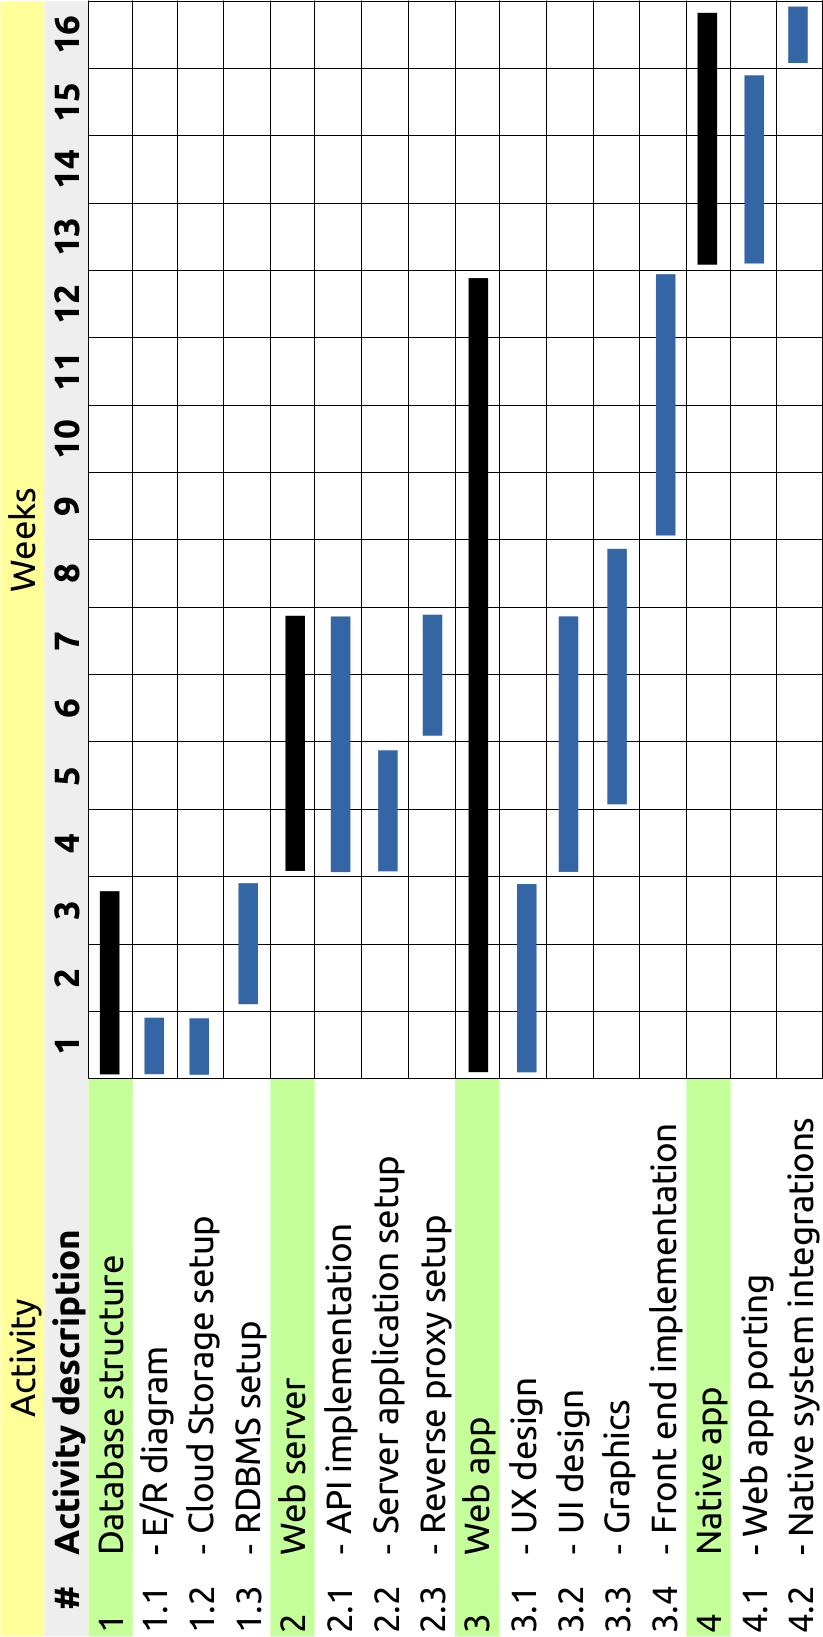
\includegraphics[origin=c,width=\textwidth,height=.95\textheight,keepaspectratio]{DD_Images/Gantt.jpg}
  \caption{\textit{Reference Gantt}}
\end{figure}